\documentclass{beamer}
\title{Progetto ICON 21/22}
\author{Francesco Bottalico}
\date{2022}
\usetheme{Copenhagen}
\usepackage{graphicx}
\usepackage{spreadtab}
\graphicspath{ {../imgs/} }
\STautoround{3}

\begin{document}

\frame{\titlepage}

\begin{frame}
	\frametitle{Introduzione}
	\begin{block}{Obiettivo}
		Migliorare modelli supervisionati e non attraverso l'estrazione di
		conoscenza aggiuntiva dal web semantico.
	\end{block}
	In particolare:
	\begin{itemize}
		\item Interrogazione di un'ontologia (DBPedia) per estrarre feature
			utili per migliorare le qualità delle predizioni
		\item Allenamento di modelli di apprendimento supervisionato visti a
			lezione (con model selection per la scelta degli iperparametri)
		\item Combinare i precedenti modelli con dei modelli di clustering
			+ background knowledge di DBPedia per migliorare ulteriormente le
			performance
	\end{itemize}
\end{frame}

\begin{frame}
	\frametitle{Features}
	Le seguenti sono le feature originali del dataset:
	\begin{columns}
		\column{0.5\textwidth}
		\begin{itemize}
			\itemsep0em
			\item \textbf{date}
			\item \textbf{price}
			\item \textbf{bedrooms}
			\item \textbf{bathrooms}
			\item \textbf{sqft\_living}
			\item \textbf{sqft\_lot}
			\item \textbf{floors}
			\item \textbf{waterfront}
			\item \textbf{view}
			\item \textbf{condition}
			\item \textbf{sqft\_above}
			\item \textbf{sqft\_basement}
			\item \textbf{yr\_built}
		\end{itemize}
		\column{0.5\textwidth}
		\begin{itemize}
			\item \textbf{yr\_renovated}
			\item \textbf{street}
			\item \textbf{city}
			\item \textbf{statezip}
			\item \textbf{country}
		\end{itemize}
		\begin{alertblock}{Feature estratte dal web semantico}
			\begin{itemize}
				\item \textbf{lat}
				\item \textbf{long}
				\item \textbf{density}
			\end{itemize}
		\end{alertblock}
	\end{columns}
\end{frame}

\begin{frame}
	\frametitle{Correlazione tra posizione e prezzo delle case}
La posizione della casa effettivamente influisce sul prezzo, mentre la densità
sembra influire meno, come si può vedere nella figura.
\begin{figure}[ht]
	\centering
	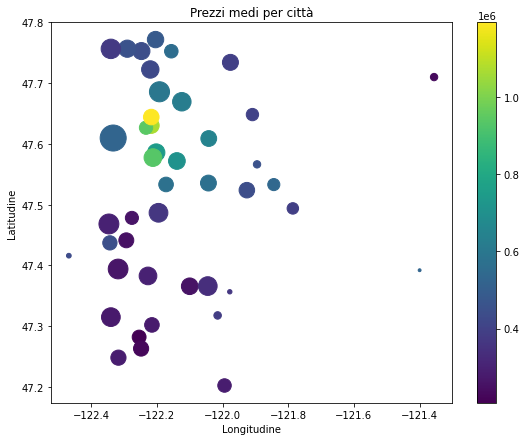
\includegraphics[scale=0.25]{cities}
	\caption{Case raggruppate per città, il colore rappresenta il prezzo
	medio delle case, la grandezza del punto mostra la densità di popolazione.
	Si nota un gruppo di città limitrofe per il quale il prezzo medio delle
	case è maggiore.}
\end{figure}
\end{frame}

\begin{frame}
	\frametitle{Preprocessing sul dataset}
	\begin{columns}
	\column{0.5\textwidth}
	\begin{block}{Preprocessing}
		\begin{enumerate}
			\item Eliminazione degli elementi con prezzo nullo
			\item Feature selection: vengono eliminate le feature \alert{date},
				\alert{street}, \alert{country}, \alert{waterfront}
			\item \alert{yr\_renovated = yr\_built} se la casa non è mai stata
				ristrutturata
			\item Rimozione degli outliers ($zscore < |2.5|$)
			\item Standardizzazione
			\item One hot encoding
		\end{enumerate}
	\end{block}
		\column{0.5\textwidth}
			\begin{figure}[ht]
				\centering
				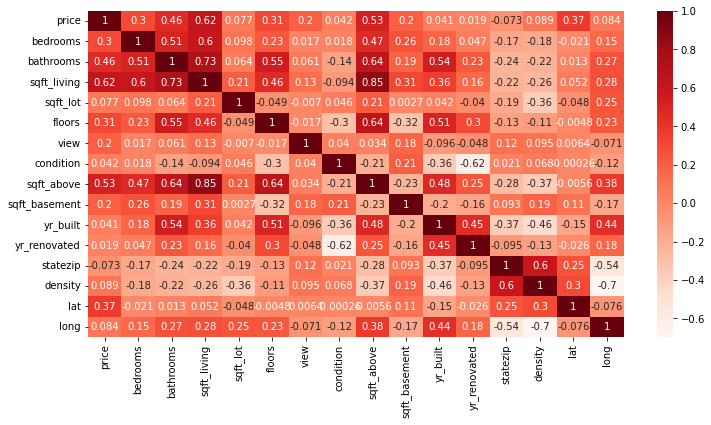
\includegraphics[scale=0.2]{correlazione.png}
			\end{figure}
			\begin{figure}[ht]
				\centering
				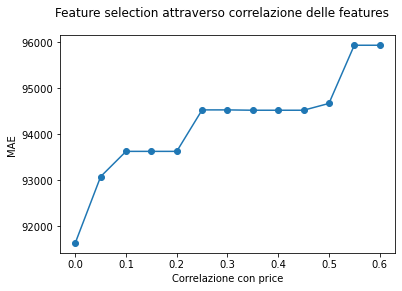
\includegraphics[scale=0.3]{selection.png}
			\end{figure}
	\end{columns}
\end{frame}

\begin{frame}
	\frametitle{Splitting del dataset}
	Il dataset viene diviso in training e testing set in due modi:
	\begin{itemize}
		\item Splitting degli elementi randomico
		\item Splitting in modo tale da avere elementi senza città in comune nel
			training e testing set. In questo modo è possibile simulare la
			situazione nella quale viene effettuata una predizione di un
			elemento in una città mai incontrata nel training. Utile per valutare
			l'utilita delle feature estratte \alert{lat} e \alert{long}.
	\end{itemize}
\end{frame}

\begin{frame}
	\frametitle{Apprendimento supervisionato}
	\fontsize{8pt}{10}
	Vengono allenati i seguenti modelli di apprendimento supervisionato, la
	model selection viene effettuata con una k-fold cross validation.
	\begin{description}
	\item[Rete neurale]
	Per la rete neurale viene effettuata la model selection su diversi parametri
	quali: algoritmo di ottimizzazione, numero di neuroni, strati e parametro per
	la regolarizzazione L2.
	\item[Regressione lineare]
	Gli iperparametri che vengono stimati dalla cross validation sono il learning
	rate, il suo metodo di aggiornamento ed il parametro di regolarizzazione
	$\alpha$. Viene provata sia la regolarizzazione L1 che la L2.
	\item[Decision tree]
	Per il decision tree la cross validation viene utilizzata per stimare parametri
	quali la massima profondità dell'albero ed il numero minimo di sample che una
	foglia deve contenere.
	\item[Random forest]
	Per la random forest vengono allenati 100 decision trees, gli iperparametri
	stimati attraverso la cross validation sono la profondità massima degli alberi
	ed il numero massimo di feature prese in considerazione durante il training.
	\item[Support vector machine]
	Nel caso della SVM vengono provate diverse funzioni kernel (per il kernel
	polinomiale si provano diversi gradi) e alcuni valori per il parametro per la
	regolarizzazione C (che è inversamente proporzionale alla forza della
	regolarizzazione).
	\end{description}
\end{frame}

\begin{frame}
	\frametitle{Model selection rete neurale}
	\begin{figure}[ht]
		\centering
		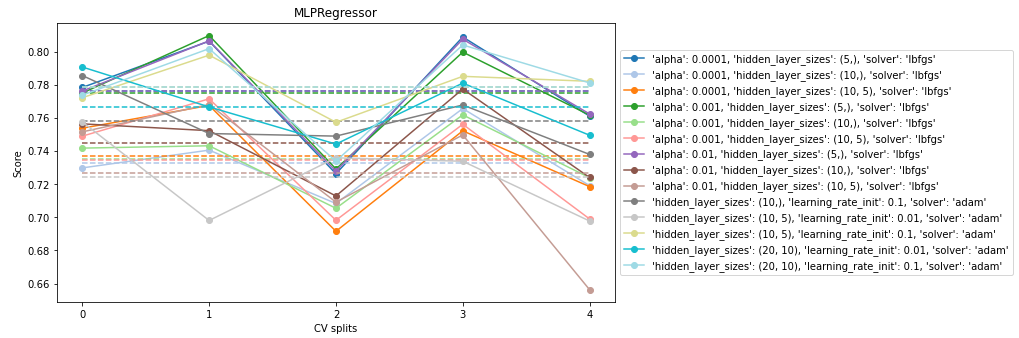
\includegraphics[width=\textwidth]{nncv.png}
		\caption{Andamento dello score sui vari fold della cross validation dati
		diversi valori per gli iperparametri. le rette tratteggiate indicano il
		valore medio.}
		\begin{alertblock}{Migliori parametri}
			solver = 'adam'\\
			hidden\_layer\_sizes=(20,10)\\
			learning\_rate\_init=0.1
		\end{alertblock}
	\end{figure}
\end{frame}

\begin{frame}
	\frametitle{Model selection regressione lineare L1 e L2}
	\begin{columns}
	\column{0.7\textwidth}
		\begin{figure}[ht]
			\centering
			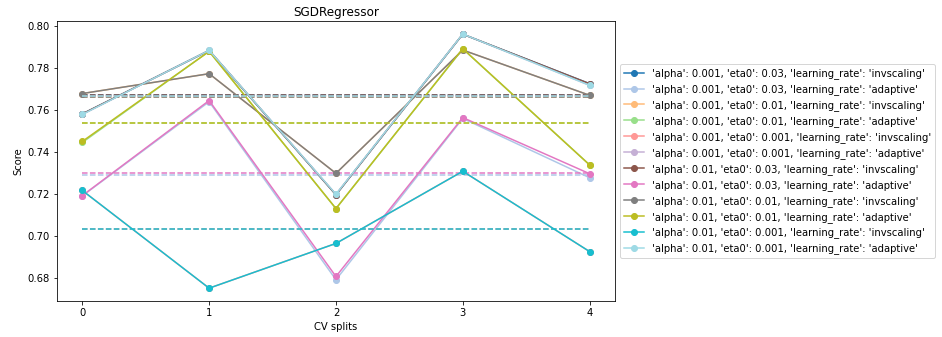
\includegraphics[width=\textwidth]{lassocv.png}
			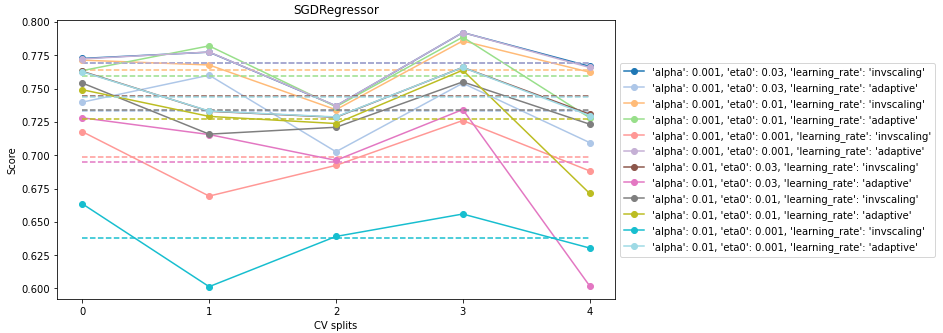
\includegraphics[width=\textwidth]{ridgecv.png}
			\caption{Score delle cross validation per la model selection dei modelli
			di regressione lineare con regolarizzazione L1 (sopra) ed L2 (sotto).}
		\end{figure}
	\column{0.3\textwidth}
		\begin{alertblock}{Migliori parametri L1}
			alpha = 0.001\\
			eta0 = 0.03\\
			learning\_rate = 'invscaling'
		\end{alertblock}
		\begin{alertblock}{Migliori parametri L2}
			alpha = 0.001\\
			eta0 = 0.03\\
			learning\_rate = 'invscaling'
		\end{alertblock}
	\end{columns}
\end{frame}

\begin{frame}
	\frametitle{Model selection decision tree}
	\begin{figure}[ht]
		\centering
		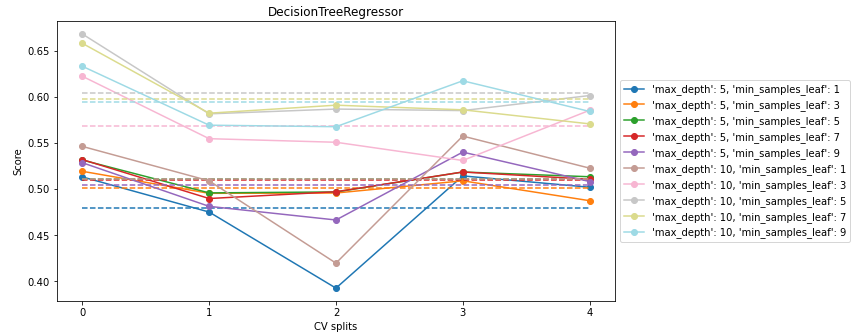
\includegraphics[width=\textwidth]{treecv.png}
		\caption{Score delle cross validation per la model selection del decision
		tree.}
	\end{figure}
	\begin{alertblock}{Migliori parametri}
		max\_depth = 10\\
		min\_samples\_leaf = 5
	\end{alertblock}
\end{frame}

\begin{frame}
	\frametitle{Model selection random forest}
	\begin{figure}[ht]
		\centering
		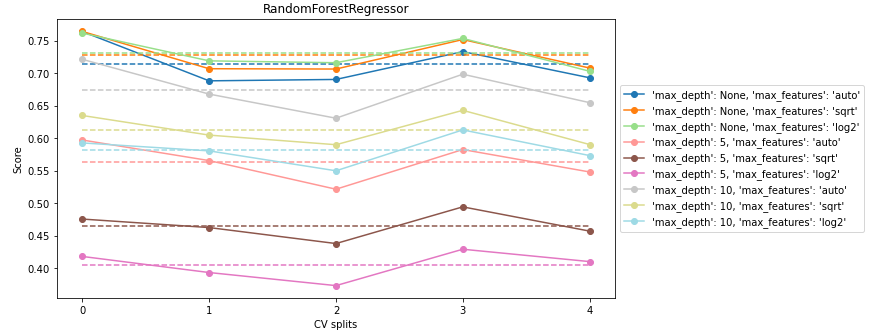
\includegraphics[width=\textwidth]{ranfcv.png}
		\caption{Score delle cross validation per la model selection del decision
		tree.}
	\end{figure}
	\begin{alertblock}{Migliori parametri}
		max\_depth = None\\
		max\_features = 'log2'
	\end{alertblock}
\end{frame}

\begin{frame}
	\frametitle{Model selection SVM}
	\begin{figure}[ht]
		\centering
		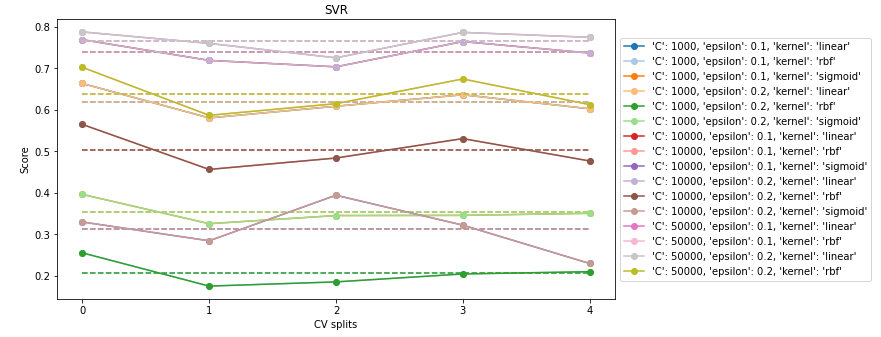
\includegraphics[width=\textwidth]{svmcv.png}
		\caption{Score delle cross validation per la model selection della support
		vector machine.}
	\end{figure}
	\begin{alertblock}{Migliori parametri}
		C = 50000\\
		kernel = 'linear'
	\end{alertblock}
\end{frame}

\begin{frame}
	\frametitle{Apprendimento non supervisionato: K-means}
	\textbf{Le predizioni dei modelli possono essere migliorate con l'utilizzo
	del clustering:}
	\begin{itemize}
		\item Dividere il training set in cluster
		\item Allenare indipendentemente un modello supervisionato su ogni cluster
		\item Per la predizione: assegnare il dato al cluster ed effettuare la
			predizione con il rispettivo modello
	\end{itemize}
\end{frame}

\begin{frame}
	\frametitle{Apprendimento non supervisionato: K-means}
	Il clustering può essere effettuato in due modi:
	\begin{itemize}
		\item K-means su tutte le features del dato $\rightarrow$ dati non 
			divisibili per $k > 2$
		\item K-means solo sulle features \alert{lat} e \alert{long} tenendo
			conto della relazione con il prezzo vista in precedenza
			$\rightarrow$ valore ottimale $k = 3$ con l'elbow method
	\end{itemize}
	\begin{figure}
		\centering
		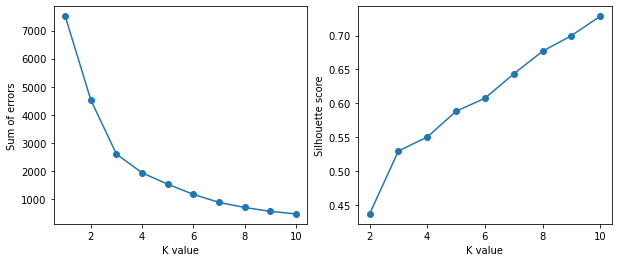
\includegraphics[width=0.8\textwidth]{kselection2.png}
		\caption{Andamento dell'errore all'aumentare di k nel secondo caso}
	\end{figure}
\end{frame}

\begin{frame}
	\frametitle{Confronto modelli - equal splitting}
	\begin{table}[ht]
		\tiny
		\centering
		\begin{spreadtab}{{tabular}{c|c|c|c|c|c|c|r|}}
			\cline{2-8}
			& @ \multicolumn{3}{|c|}{Original data} & @ \multicolumn{3}{c|}{Extended data} & \\
			\cline{2-7}
			& @ R2 & @ RMSE & @ MAE & @ R2 & @ RMSE & @ MAE & @ decr. MAE\\
			\hline
			@ \multicolumn{1}{|c|}{Dummy} & -0.003 & 253592.36 & 191642.73 &
			-0.003 & 253592.36 & 191642.73 & \textbf{:={[-4,0]*100/[-1,0]-100}}\%\\
			\hline
			@ \multicolumn{1}{|c|}{Rete neurale} & 0.835 & 102802.54 & 67716.71 &
			0.843 & 100257.86 & 66375.14 & \textbf{:={[-4,0]*100/[-1,0]-100}}\%\\
			\hline
			@ \multicolumn{1}{|c|}{Lasso} & 0.820 & 107530.43 & 71892.61 &
			0.818 & 107884.67 & 72514.84 & \textbf{:={[-4,0]*100/[-1,0]-100}}\%\\
			\hline
			@ \multicolumn{1}{|c|}{Ridge} & 0.811 & 109967.49 & 73629.67 &
			0.812 & 109665.55 & 72766.01 & \textbf{:={[-4,0]*100/[-1,0]-100}}\%\\
			\hline
			@ \multicolumn{1}{|c|}{Decision tree} & 0.688 & 141346.10 & 100310.09 &
			0.711 & 136167.39 & 91516.67 & \textbf{:={[-4,0]*100/[-1,0]-100}}\%\\
			\hline
			@ \multicolumn{1}{|c|}{Random forest} & 0.772 & 120975.81 & 77201.70 &
			0.785 & 117388.42 & 74131.08 & \textbf{:={[-4,0]*100/[-1,0]-100}}\%\\
			\hline
			@ \multicolumn{1}{|c|}{SVM} & 0.800 & 113336.14 & 70691.88 &
			0.796 & 114286.55 & 71563.63 & \textbf{:={[-4,0]*100/[-1,0]-100}}\%\\
			\hline
		\end{spreadtab}
		\label{tab:eq}
		\caption{Risultati predizioni usando la funzione di equal splitting.}
	\end{table}
	\begin{table}[ht]
		\tiny
		\centering
		\begin{tabular}{c|c|c|c|c|c|c|r|}
			\cline{2-8}
			& \multicolumn{2}{|c}{\textbf{Cluster 1} (304/751)}
			& \multicolumn{2}{|c|}{\textbf{Cluster 2} (206/751)}
			& \multicolumn{2}{c|}{\textbf{Cluster 3} (241/751)} & \\
			\cline{2-7}
			& RMSE & MAE & RMSE & MAE & RMSE & MAE & Tot MAE \\
			\hline
			\multicolumn{1}{|c|}{Rete neurale} & 120621.8 & 84109.2 & 54167.9 &
			36626.5 & 107014.3 & 70194.7 & \textbf{66619.4}\\
			\hline
			\multicolumn{1}{|c|}{Lasso}	& 122742.4 & 85282.6 & 53754.3 &
			37012.4 & 110568.8 & 72466.9 & \textbf{67929.4}\\
			\hline
			\multicolumn{1}{|c|}{Ridge} & 126733.2 & 86639.7 & 54087.4 &
			36824.5 & 111961.8 & 73232.2 & \textbf{68672.8}\\
			\hline
			\multicolumn{1}{|c|}{Decision tree} & 175090.9 & 125769.1 & 71349.5 &
			48866.8 & 139656.1 & 86026.7 & \textbf{91921.2}\\
			\hline
			\multicolumn{1}{|c|}{Random forest} & 133296.1 & 92910.0 & 57140.5 &
			40125.2 & 130805.0 & 76968.6 & \textbf{73315.4}\\
			\hline
			\multicolumn{1}{|c|}{SVM} & 120161.8 & 82193.3 & 55079.3 &
			36726.1 & 117846.7 & 75034.6 & \textbf{67424.3}\\
			\hline
		\end{tabular}
		\caption{Risultati delle predizioni combinando apprendimento supervisionato
		e K-means. \alert{Lasso}, \alert{SVM} e \alert{Ridge} hanno miglioramenti.}
	\end{table}
\end{frame}

\begin{frame}
	\frametitle{Confronto modelli - different cities splitting}
\begin{table}[ht]
	\tiny
	\centering
	\begin{spreadtab}{{tabular}{c|c|c|c|c|c|c|r|}}
		\cline{2-8}
		& @ \multicolumn{3}{|c|}{Original data} & @ \multicolumn{3}{c|}{Extended data} & \\
		\cline{2-7}
		& @ R2 & @ RMSE & @ MAE & @ R2 & @ RMSE & @ MAE & @ decr. MAE\\
		\hline
		@ \multicolumn{1}{|c|}{Dummy} & -0.000 & 241153.04 & 189087.16
		& -0.000 & 241153.04 & 189087.16 & \textbf{:={[-4,0]*100/[-1,0]-100}}\%\\
		\hline
		@ \multicolumn{1}{|c|}{Rete neurale} & 0.117 & 226651.86 & 182441.63
		& 0.392 & 188103.04 & 141451.75 & \textbf{:={[-4,0]*100/[-1,0]-100}}\%\\
		\hline
		@ \multicolumn{1}{|c|}{Lasso} & 0.477 & 174465.26 & 137111.43
		& 0.600 & 152593.23 & 109693.36 & \textbf{:={[-4,0]*100/[-1,0]-100}}\%\\
		\hline
		@ \multicolumn{1}{|c|}{Ridge} & 0.487 & 172658.18 & 134693.90
		& 0.600 & 152514.45 & 109608.88 & \textbf{:={[-4,0]*100/[-1,0]-100}}\%\\
		\hline
		@ \multicolumn{1}{|c|}{Decision tree} & -0.211 & 265360.75 & 197765.79
		& 0.542 & 163191.47 & 108231.19 & \textbf{:={[-4,0]*100/[-1,0]-100}}\%\\
		\hline
		@ \multicolumn{1}{|c|}{Random forest} & 0.368 & 191684.83 & 149244.86
		& 0.630 & 146678.88 & 104214.31 & \textbf{:={[-4,0]*100/[-1,0]-100}}\%\\
		\hline
		@ \multicolumn{1}{|c|}{SVM} & 0.439 & 180650.80 & 136976.35
		& 0.599 & 152661.49 & 106088.53 & \textbf{:={[-4,0]*100/[-1,0]-100}}\%\\
		\hline
	\end{spreadtab}
	\caption{Risultati predizioni con nuove città durante il testing, il
	miglioramento sui dati "estesi" è notevole.}
\end{table}
\begin{table}[ht]
	\tiny
	\centering
	\begin{tabular}{c|c|c|c|c|c|c|r|}
		\cline{2-8}
		& \multicolumn{2}{|c}{\textbf{Cluster 1} (95/671)}
		& \multicolumn{2}{|c|}{\textbf{Cluster 2} (354/671)}
		& \multicolumn{2}{c|}{\textbf{Cluster 3} (222/671)} & \\
		\cline{2-7}
		& RMSE & MAE & RMSE & MAE & RMSE & MAE & Tot MAE \\
		\hline
		\multicolumn{1}{|c|}{Rete neurale} & 329103.3 & 265676.8 & 138318.8
		& 106167.8 & 64009.5 & 45005.8 & \textbf{108515.6} \\
		\hline
		\multicolumn{1}{|c|}{Lasso} & 246069.3 & 209740.8 & 147408.7
		& 100309.3 & 65457.8 & 46995.7 & \textbf{98163.8} \\
		\hline
		\multicolumn{1}{|c|}{Ridge} & 241350.0 & 205236.3 & 147258.7
		& 100224.0 & 65334.7 & 46834.0 & \textbf{97427.6} \\
		\hline
		\multicolumn{1}{|c|}{Decision tree} & 279222.8 & 195405.9 & 177526.5
		& 125350.3 & 83347.6 & 57663.3 & \textbf{112874.5} \\
		\hline
		\multicolumn{1}{|c|}{Random forest} & 231919.2 & 176273.3 & 156945.9
		& 107479.8 & 68201.1 & 44938.3 & \textbf{96527.7} \\
		\hline
		\multicolumn{1}{|c|}{SVM} & 162850.3 & 123706.7 & 141990.1
		& 99907.8 & 64456.9 & 42933.3 & \textbf{84427.3} \\
		\hline
	\end{tabular}
	\caption{Risultati delle predizioni combinando apprendimento supervisionato
	e K-means, \alert{Lasso} ha un incremento notevole delle performance.}
\end{table}
\end{frame}

\end{document}
